
\documentclass{article}
\usepackage[headheight=20pt, margin=1.0in, top=1.2in]{geometry}
\usepackage{amsmath, amssymb, amsthm, thmtools, tcolorbox, array, graphicx, makeidx, cancel, multirow, fancyhdr, xypic, color, nicefrac, rotating, multicol, caption, subcaption, xcolor, tikz, tikz-3dplot, tikz-cd, pgfplots, import, enumitem, calc, booktabs, wrapfig, siunitx, hyperref,float}
\hypersetup{colorlinks=true,linkcolor=blue}
\usepackage[all]{xy}
\usepackage{esint}
\setlength{\parindent}{0in}
\sisetup{per-mode = symbol}
\usetikzlibrary{calc,arrows,svg.path,decorations.markings,patterns,matrix,3d,fit}
\usepgfplotslibrary{groupplots}
\pgfplotsset{compat=newest}
\newtcolorbox{mydefbox}[2][]{colback=red!5!white,colframe=red!75!black,fonttitle=\bfseries,title=#2,#1}
\newtcolorbox{mythmbox}[2][]{colback=gray!5!white,colframe=gray!75!black,fonttitle=\bfseries,title=#2,#1}
\newtcolorbox{myexamplebox}[2][]{colback=green!5!white,colframe=green!75!black,fonttitle=\bfseries,title=#2,#1}
\newtcolorbox{mypropbox}[2][]{colback=blue!5!white,colframe=blue!75!black,fonttitle=\bfseries,title=#2,#1}
\declaretheoremstyle[headfont=\color{blue}\normalfont\bfseries,]{colored}
\theoremstyle{definition}
\newtheorem{theorem}{Theorem}
\newtheorem{corollary}[theorem]{Corollary}
\newtheorem{lemma}[theorem]{Lemma}
\newtheorem{proposition}[theorem]{Proposition}
\newtheorem{problem}[theorem]{Problem}
\newtheorem{definition}[theorem]{Definition}
\newtheorem{exercise}[theorem]{Exercise}
\newtheorem{example}[theorem]{Example}
\newtheorem{solution}[theorem]{Solution}
\newtheorem*{thm}{Theorem}
\newtheorem*{lem}{Lemma}
\newtheorem*{prob}{Problem}
\newtheorem*{exer}{Exercise}
\newtheorem*{prop}{Proposition}
\def\R{\mathbb{R}}
\def\F{\mathbb{F}}
\def\Q{\mathbb{Q}}
\def\C{\mathbb{C}}
\def\N{\mathbb{N}}
\def\Z{\mathbb{Z}}
\def\Ra{\Rightarrow}
\def\e{\epsilon}
\newcommand{\typo}[1]{{\color{red}{#1}}}
\newcommand\thedate{\today}
\newcommand{\mb}{\textbf}
\newcommand{\norm}[2]{\|{#1}\|_{#2}}
\newcommand{\normm}[1]{\|#1\|}
\newcommand{\mat}[1]{\begin{bmatrix} #1 \end{bmatrix}}
\newcommand{\eqtext}[1]{\hspace{3mm} \text{#1} \hspace{3mm}}
\newcommand{\set}[1]{\{#1\}}
\newcommand{\inte}{\textrm{int}}
\newcommand{\ra}{\rightarrow}
\newcommand{\minv}{^{-1}}
\newcommand{\tx}[1]{\text{ {#1} }}
\newcommand{\abs}[1]{|#1|}
\newcommand{\mc}[1]{\mathcal{#1}}
\newcommand{\uniflim}{\mathop{\mathrm{unif\lim}}}
\newcommand{\notimplies}{\mathrel{{\ooalign{\hidewidth$\not\phantom{=}$\hidewidth\cr$\implies$}}}}
\pagestyle{fancy}
\fancyhf{}
\fancyhead[L]{Title of the Document}
\fancyhead[C]{}
\fancyhead[R]{\thepage}
\fancyfoot[L]{}
\fancyfoot[C]{}
\fancyfoot[R]{}
\renewcommand{\headrulewidth}{0.4pt}
\renewcommand{\footrulewidth}{0.4pt}
\numberwithin{equation}{section}
% Increase spacing between paragraphs
\setlength{\parskip}{1em}
% Increase spacing before and after sections
\usepackage{titlesec}
\titlespacing*{\section}{0pt}{3ex plus 1ex minus .2ex}{2ex plus .2ex}
\titlespacing*{\subsection}{0pt}{2ex plus 1ex minus .2ex}{1ex plus .2ex}
\titlespacing*{\subsubsection}{0pt}{1ex plus 1ex minus .2ex}{1ex plus .2ex}
\title{\textbf{Title of the Document}}
\author{Author Name}
\date{\today}
\begin{document}
\maketitle
\tableofcontents
\newpage
\section{Exercises}

\begin{enumerate}
    \item Let $(X, d)$ be a metric space and $S \subseteq X$. Show that $\partial S = \emptyset$ if and only if $S$ is both open and closed.
    \item Show that for an arbitrary choice of $a, b, r \in \mathbb{R}$, the closed disk $(x-a)^2 + (y - b)^2 \leq r^2$ is in a bounded set in $\mathbb{R}^2$.
    \item Let $(X, d)$ be a metric space and for $x, y \in X$. Show that if $d(x, y) < \epsilon$ for every $\epsilon > 0$, then $x = y$.
\end{enumerate}

\noindent (i) Assume $S \not= \emptyset$. Then $\exists x \in S$, such that $x \notin \partial S$*. Then $x \in S^{int}$ and there exists $\epsilon > 0$ such that $B_{\epsilon}(x) \subseteq S$. 

However, by $x \notin \partial S$, this value of $\epsilon > 0$ implies $B_{\epsilon}(x) \cap S = \emptyset$, which is a contradiction, implying our assumption that $x \in S \cap S^{int}$ must be false and $\partial S \cap S^{int} = \emptyset$. 

\noindent (iii) A set $S$ is bounded iff $\exists M > 0$, such that $d(x, y) \leq M$, $\forall x, y \in S$

Let $a, b, r \in \mathbb{R}$. 

$\delta = \{(x, y) \in \mathbb{R} | (x-a)^2 + (y-b)^2 \leq r^2 \} \implies x^2 - 2ax + a^2 + y^2 -2by + b^2 \leq r^2$

$\implies x^2 - 2ax + y^2 - 2by \leq r^2 - a^2 - b^2 \implies x^2 - 2ax + y^2 - 2by \leq r^2 - a^2 - b^2 + 2ax + 2by$

$\implies x^2 + y^2 \leq r^2 - a^2 - b^2 + 2ax + 2by$

Need to show $x^2$ is bounded,

$(x-a)^2 \leq r^2 \implies |x-a| \leq |r| \implies |x-a| \leq |r| + |a|$

$\implies |x| = |x-a+a| \leq |x-a|+|a| \leq |r| + |a|$

$\implies |x| \leq |x-a+a| \leq |x-a|+|a| \leq |r| + |a|$

\begin{align*}
&\Rightarrow |y| \leq r + |a| \\
&\Rightarrow y^2 \leq (r + |a|)^2 \\
\end{align*}

\text{Same for } x, x^2 \leq (r + |b|)^2

$\forall z = (x,y) \in D_{r, (a,b)}$

$\|z\| = \sqrt{x^2 + y^2} \leq \sqrt{(r+|a|)^2 + (r+|b|)^2}$

Thus if \(\sqrt{(r+|a|)^2 + (r+|b|)^2}\), the bound holds.

$
\#\text{IS named boundless} = \text{distance boundedness.}
$

Let \( x = (x_1, x_2), y = (y_1, y_2) \in D_{r,(a,b)} \)

$
z_i \in \{x_i, y_i\}
$

$
(x_i - a)^2 + (x_i - b)^2 = r^2
$

$
\Rightarrow d((x_i, b)) = \sqrt{(x_i - a)^2 + (x_i - b)^2} \leq r
$

$
\Rightarrow d((x, y)) \leq d((x, (a,b))) + d(y, (a,b))
$

$
= \sqrt{(x_i - a)^2 + (x_i - b)^2} + \sqrt{(y_i - a)^2 + (y_i - b)^2} \leq r + r = 2r
$

\noindent (iii) \textbf{Suppose that $x \neq y$. Then $d(x,y) \neq 0$. Thus if we choose $\epsilon = d(x,y) \Rightarrow \epsilon > 0$ but $d(x,y) \notin \epsilon$. (contradiction).}

\textbf{(contradiction)} Suppose $x \neq y$ and so $d(x,y) \neq 0$. 

Choose $\epsilon > 0$ so that $\epsilon = d(x,y)$. Then we must have 
$ d(x,y) < \epsilon = \frac{d(x,y)}{2}, $
which is a contradiction, as this implies 
$ d(x,y) = \frac{d(x,y)}{2} $

If $d(x,y) < \frac{d(x,y)}{2}$ 

So $d(x,y) \leq s \epsilon = \frac{\epsilon}{2} $

Thus $ \frac{\epsilon}{2} < \epsilon $

\subsubsection*{(iv)}

Let $(V, || \cdot ||)$ be a normed vsp.

Then let $r > 0$ and $x \in V$. Then 
$ B_r(x) = \left\{ u \in V \mid d(x,u) < r \right\} $
$ B_{r + || x ||}(0) = \left\{ v \in V \mid d(0,u) < r + || x || \right\} $

$
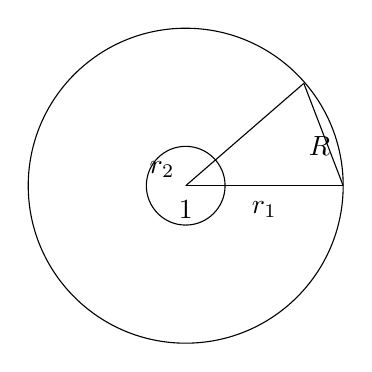
\begin{tikzpicture}
\draw (0,0) circle (2cm);
\draw (0,0) -- (2,0);
\draw (2,0) -- (1.5,1.3);
\draw (1.5,1.3) -- (0,0);
\draw (0,0) circle (0.5cm);
\node at (-0.3, 0.2) {$r_2$};
\node at (1, -0.3) {$r_1$};
\node at (0, -0.3) {$1$};
\node at (1.7, 0.5) {$R$};
\end{tikzpicture}
$

Let $y \in B_r(x)$

$ d(0,y) \leq d(0,x) + d(x,y) $

$ \leq || x || + r $

\Rightarrow 
$ B_r(x) \subseteq B_{r + ||  x  ||}(0) $

(v) Suppose $S$ is bounded. Then $\exists M \in \mathbb{R}$ such that $\forall x \in S || x || \leq M$ 

$ (Equal to \exists M \in \mathbb{R} : \forall x \in V ) \in S \subseteq B_M(0) $\end{document}